\section{先行研究}

\subsection{クラスタリング}
クラスタリングとはデータを教師なし学習により任意の数のクラスタに分ける手法である.
多くのクラスタリング手法においては,データの類似度をユークリッド距離やマンハッタン距離などの
距離尺度によって定義し,それによってクラスタを抽出する.
クラスタリングはデータ解析,データマイニング,パターン認識など様々な分野で用いられる.

\subsection{K-means}
K-means$^{1)}$は,多次元空間上のデータ点集合について,各データが属するクラスタを同定する最もよく使われるクラスタリング手法の一つである.
% K-meansは,以下の2つの手順を繰り返すことでクラスタリングを行う.
% \begin{enumerate}
%   \item 各データ点とデータ点の距離を求め,各データ点を最も近いセントロイドのクラスタに割り当てる.
%   \item クラスタに所属するデータの平均を新たなセントロイドとする.
% \end{enumerate}
% セントロイドが移動しなくなったらクラスタリングを終了する.

$D$次元空間上の確率変数$x$の$N$個の観測点で構成されるデータ集合
$\{\vector{x}_1, \vector{x}_2, \cdots, \vector{x}_N\}$があると仮定する.
このデータ集合を$K$個のクラスタに分割することを考える.
直感的には,クラスタとは,その内部のデータ点間の距離が外部のデータとの距離と比較して小さいテータのグループであるとみなせる.
ここで,セントロイド$\vector{\mu}_k$を導入する.
K-meansはベクトルの集合$\{\vector{\mu}_k\}$だけでなく,全データ点をうまくクラスタに対応させ,
各データ点から $\vector{\mu}_k$をへの二乗距離の総和を最小にすることで,クラスタリングを行う.

ここで,各データ点$\vector{x}_n$に対し,対応する2値指示変数$r_{nk} \in \{0, 1\}\ (k = 1, \cdots, K)$を定める.
これは,そのデータ点$\vector{x}_n$がクラスタ$k$に割り当てられるかを表す変数である.
すなわち,データ点$\vector{x}_n$がクラスタ$k$に割り当てられる場合は$r_{nk}=1$とし,
$j \not= k$については,$r_{nk}=0$とする.これは,1-of-K符号化法として知られている.

次に,次の目的関数$J$を定義する.

\begin{align}
  \label{eq:J-func}
  J = \sum_{n=1}^{N} \sum_{k=1}^{K} r_{nk} || {\displaystyle \vector{x}_n - \vector{\mu}_k} || ^2
\end{align}

これは,歪み尺度と呼ばれ,各データ点からそれらが割り当てられたベクトル$\vector{\mu}_k$までの二乗距離の総和を表している.
K-meansによるクラスタリングは,$J$を最小にする$\{r_{nk}\}$と$\{\vector{\mu}_k\}$の値を求めることである.

\begin{figure}[htbp]
  \begin{minipage}{0.33\hsize}
    \begin{center}
      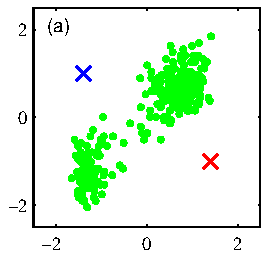
\includegraphics[width=40mm]{img/kmeans/Figure91a.pdf}
    \end{center}
  \end{minipage}
  \begin{minipage}{0.33\hsize}
    \begin{center}
      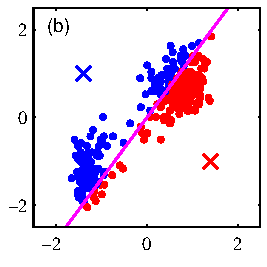
\includegraphics[width=40mm]{img/kmeans/Figure91b.pdf}
    \end{center}
  \end{minipage}
  \begin{minipage}{0.33\hsize}
    \begin{center}
      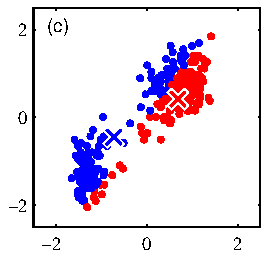
\includegraphics[width=40mm]{img/kmeans/Figure91c.pdf}
    \end{center}
  \end{minipage}\\
  \begin{minipage}{0.33\hsize}
    \begin{center}
      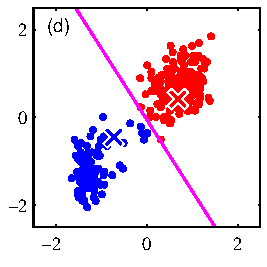
\includegraphics[width=40mm]{img/kmeans/Figure91d.pdf}
    \end{center}
  \end{minipage}
  \begin{minipage}{0.33\hsize}
    \begin{center}
      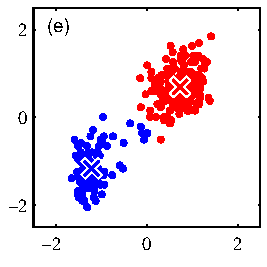
\includegraphics[width=40mm]{img/kmeans/Figure91e.pdf}
    \end{center}
  \end{minipage}
  \begin{minipage}{0.33\hsize}
    \begin{center}
      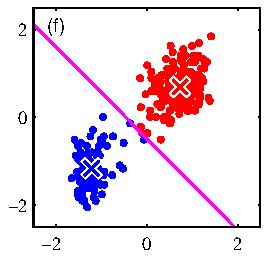
\includegraphics[width=40mm]{img/kmeans/Figure91f.pdf}
    \end{center}
  \end{minipage}\\
  \begin{minipage}{0.33\hsize}
    \begin{center}
      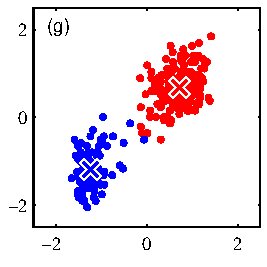
\includegraphics[width=40mm]{img/kmeans/Figure91g.pdf}
    \end{center}
  \end{minipage}
  \begin{minipage}{0.33\hsize}
    \begin{center}
      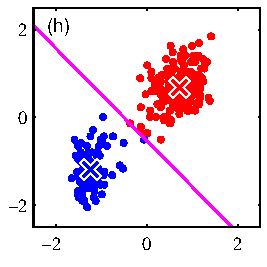
\includegraphics[width=40mm]{img/kmeans/Figure91h.pdf}
    \end{center}
  \end{minipage}
  \begin{minipage}{0.33\hsize}
    \begin{center}
      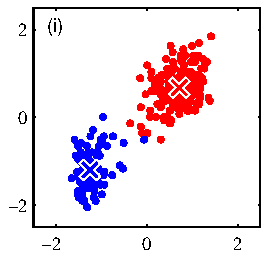
\includegraphics[width=40mm]{img/kmeans/Figure91i.pdf}
    \end{center}
  \end{minipage}
  \caption{K-meansの動作}
  \label{fig:k-means}
\end{figure}

\figurenum{fig:k-means}にK-meansによるクラスタリングの具体例を示す.
K-meansでは,$r_{nk}$と$\vector{\mu}_k$をそれぞれ最適化する2つのステップを
交互に繰り返す手続きでクラスタリングを実現する.

最初に,$\vector{\mu}_k$の初期値を選ぶ(a).
次に,最初のフェーズで$\vector{\mu}_k$を固定しつつ,$r_{nk}$について$J$を最小化する(b).
第二フェーズでは,$r_{nk}$を固定しつつ,$\vector{\mu}_k$について$J$を最小化する(c).
そして,このような二段階最適化を収束するように繰り返す.

まず$r_{nk}$の決定を考える.
\eqref{eq:J-func}における$J$は$r_{nk}$についての線形関数なので,最適化は代数的に解くことができる.
異なる$n$を含む項は互いに独立である.よって,各$n$について別々に$r_{nk}=1$としたときに,
$||\vector{x}_n - \vector{\mu}_k||^2$が最小になるような$k$の値に対して$r_{nk}$を選んで1とおけばよい(\eqref{eq:rnk}).
つまり,単純に$n$番目のデータ点の中心がそれに最も近いクラスタ中心に割り当てるのである.
\begin{align}
  \label{eq:rnk}
  r_{nk} = \left\{
    \begin{array}{l}
      1\ \ k = \arg\min_j ||\vector{x}_n - \vector{\mu}_j||のとき\\
      0\ \ それ以外
    \end{array}
  \right.
\end{align}

次に,$r_{nk}$を固定したもとで$\vector{\mu}_k$の最適化を考える.
対象関数$J$は$\vector{\mu}_k$の二次関数であり,次のように$\vector{\mu}_k$に関する偏微分を0とおく事で最小化できる
(\eqref{eq:mu-dif}).
\begin{align}
  \label{eq:mu-dif}
  2\sum_{n=1}^n r_{nk}(\vector{x}_n - \vector{\mu}_k) = 0
\end{align}

これを$\vector{\mu}_k$についてとくと,\eqref{eq:mu}を得る.
\begin{align}
  \label{eq:mu}
  \vector{\mu}_k = \frac{\sum_n r_{nk}\vector{x}_n}{\sum_n r_{nk}}
\end{align}

この式の分母は$k$番目のクラスタに割り当てられたデータの数に等しい.
それゆえこの式は$\vector{\mu}_k$は$k$番目のクラスタに割り当てられた全てのデータ店$\vector{x}_n$の
平均値と置いているものとして単純に解釈することができる.


K-meansによるクラスタリングは,事前にクラスタ数を指定することによりクラスタリングを行う.
したがって,クラスタ数が未知の場合,K-meansを用いることはできない.

